\begin{enumerate}[label=\thechapter.\arabic*,ref=\thechapter.\theenumi]
\numberwithin{equation}{enumi}
\numberwithin{figure}{enumi}
\numberwithin{table}{enumi}
\item
Find the maximum and minimum values of  
	\begin{enumerate}
\item Find the minimum value of the function $f\brak{x} = \brak{2x-1}^2 + 3$ using Gradient Descent method. \\ 

\solution 
\label{12/6/5/1/1/2}
\iffalse
\documentclass[12pt]{article}
\usepackage{graphicx}
\usepackage[none]{hyphenat}
\usepackage{graphicx}
\usepackage{listings}
\usepackage[english]{babel}
\usepackage{graphicx}
\usepackage{caption} 
\usepackage{booktabs}
\usepackage{array}
\usepackage{amssymb} % for \because
\usepackage{amsmath}   % for having text in math mode
\usepackage{extarrows} % for Row operations arrows
\usepackage{listings}
\lstset{
  frame=single,
  breaklines=true
}
\usepackage{hyperref}
\usepackage{mathtools}

%Following 2 lines were added to remove the blank page at the beginning
\usepackage{atbegshi}% http://ctan.org/pkg/atbegshi
\AtBeginDocument{\AtBeginShipoutNext{\AtBeginShipoutDiscard}}


%New macro definitions
\newcommand{\mydet}[1]{\ensuremath{\begin{vmatrix}#1\end{vmatrix}}}
\providecommand{\brak}[1]{\ensuremath{\left(#1\right)}}
\providecommand{\sbrak}[1]{\ensuremath{{}\left[#1\right]}}
\providecommand{\norm}[1]{\left\lVert#1\right\rVert}
\providecommand{\abs}[1]{\left\vert#1\right\vert}
\newcommand{\solution}{\noindent \textbf{Solution: }}
\newcommand{\myvec}[1]{\ensuremath{\begin{pmatrix}#1\end{pmatrix}}}
\let\vec\mathbf


\begin{document}

\begin{center}
\title{\textbf{Convex Optimization}}
\date{\vspace{-5ex}} %Not to print date automatically
\maketitle
\end{center}
\setcounter{page}{1}

\section{12$^{th}$ Maths - Chapter 6}
This is Problem-1(i) from Exercise 6.5
\begin{enumerate}
		\fi
The given function has a minimum value as shown in Figure \ref{fig:12/6/5/1/1/2Fig1}.  
\begin{align}
        \label{eq:12/6/5/1/1/2Eq1}
	f^\prime\brak{x} &= 8x-4 
\end{align}
The minimum value of the function is calculated using Gradient Descent method as below 
\begin{align}
	\label{eq:12/6/5/1/1/2grad_des}
	x_{n+1} &= x_n - \alpha \nabla f\brak{x_n}
\end{align}
Choosing
\begin{enumerate}
\item $\alpha$ = 0.001
\item precision = 0.0000001
\item n = 10000000 
\item $x_0$ = -5 
\end{enumerate}
\begin{align}
	x_{min} &= \frac{1}{2}, f\brak{x}_{min} = 3 
\end{align}
\begin{figure}[!h]
	\begin{center}
		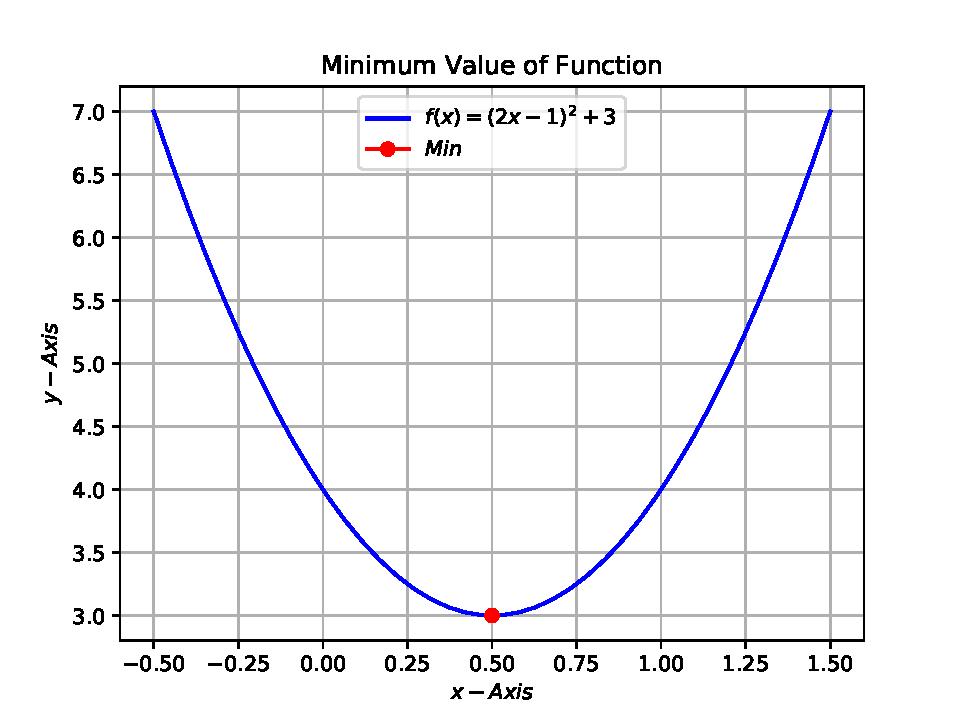
\includegraphics[width=\columnwidth]{12/6/5/1/1/2/figs/Gradient.pdf}
	\end{center}
\caption{}
\label{fig:12/6/5/1/1/2Fig1}
\end{figure}

	\end{enumerate}
\iffalse
\item
\label{12/6/5/2}
%\iffalse
\documentclass[journal,12pt,twocolumn]{IEEEtran}
\usepackage{setspace}
\usepackage{gensymb}
\usepackage{xcolor}
\usepackage{caption}
\singlespacing
\usepackage{siunitx}
\usepackage[cmex10]{amsmath}
\usepackage{mathtools}
\usepackage{hyperref}
\usepackage{amsthm}
\usepackage{mathrsfs}
\usepackage{txfonts}
\usepackage{stfloats}
\usepackage{cite}
\usepackage{cases}
\usepackage{subfig}
\usepackage{longtable}
\usepackage{multirow}
\usepackage{enumitem}
\usepackage{bm}
\usepackage{mathtools}
\usepackage{listings}
\usepackage{tikz}
\usetikzlibrary{shapes,arrows,positioning}
\usepackage{circuitikz}
\renewcommand{\vec}[1]{\boldsymbol{\mathbf{#1}}}
\DeclareMathOperator*{\Res}{Res}
\renewcommand\thesection{\arabic{section}}
\renewcommand\thesubsection{\thesection.\arabic{subsection}}
\renewcommand\thesubsubsection{\thesubsection.\arabic{subsubsection}}

\renewcommand\thesectiondis{\arabic{section}}
\renewcommand\thesubsectiondis{\thesectiondis.\arabic{subsection}}
\renewcommand\thesubsubsectiondis{\thesubsectiondis.\arabic{subsubsection}}
\hyphenation{op-tical net-works semi-conduc-tor}

\lstset{
language=Python,
frame=single, 
breaklines=true,
columns=fullflexible
}
\begin{document}
\theoremstyle{definition}
\newtheorem{theorem}{Theorem}[section]
\newtheorem{problem}{Problem}
\newtheorem{proposition}{Proposition}[section]
\newtheorem{lemma}{Lemma}[section]
\newtheorem{corollary}[theorem]{Corollary}
\newtheorem{example}{Example}[section]
\newtheorem{definition}{Definition}[section]
\newcommand{\BEQA}{\begin{eqnarray}}
\newcommand{\EEQA}{\end{eqnarray}}
\newcommand{\define}{\stackrel{\triangle}{=}}
\newcommand{\myvec}[1]{\ensuremath{\begin{pmatrix}#1\end{pmatrix}}}
\newcommand{\mydet}[1]{\ensuremath{\begin{vmatrix}#1\end{vmatrix}}}
\bibliographystyle{IEEEtran}
\providecommand{\nCr}[2]{\,^{#1}C_{#2}} % nCr
\providecommand{\nPr}[2]{\,^{#1}P_{#2}} % nPr
\providecommand{\mbf}{\mathbf}
\providecommand{\pr}[1]{\ensuremath{\Pr\left(#1\right)}}
\providecommand{\qfunc}[1]{\ensuremath{Q\left(#1\right)}}
\providecommand{\sbrak}[1]{\ensuremath{{}\left[#1\right]}}
\providecommand{\lsbrak}[1]{\ensuremath{{}\left[#1\right.}}
\providecommand{\rsbrak}[1]{\ensuremath{{}\left.#1\right]}}
\providecommand{\brak}[1]{\ensuremath{\left(#1\right)}}
\providecommand{\lbrak}[1]{\ensuremath{\left(#1\right.}}
\providecommand{\rbrak}[1]{\ensuremath{\left.#1\right)}}
\providecommand{\cbrak}[1]{\ensuremath{\left\{#1\right\}}}
\providecommand{\lcbrak}[1]{\ensuremath{\left\{#1\right.}}
\providecommand{\rcbrak}[1]{\ensuremath{\left.#1\right\}}}
\theoremstyle{remark}
\newtheorem{rem}{Remark}
\newcommand{\sgn}{\mathop{\mathrm{sgn}}}
\newcommand{\rect}{\mathop{\mathrm{rect}}}
\newcommand{\sinc}{\mathop{\mathrm{sinc}}}
\providecommand{\abs}[1]{\left\vert#1\right\vert}
\providecommand{\res}[1]{\Res\displaylimits_{#1}} 
\providecommand{\norm}[1]{\left\Vert#1\right\Vert}
\providecommand{\mtx}[1]{\mathbf{#1}}
\providecommand{\mean}[1]{E\left[ #1 \right]}
\providecommand{\fourier}{\overset{\mathcal{F}}{ \rightleftharpoons}}
\providecommand{\ztrans}{\overset{\mathcal{Z}}{ \rightleftharpoons}}
\providecommand{\system}[1]{\overset{\mathcal{#1}}{ \longleftrightarrow}}
\newcommand{\solution}{\noindent \textbf{Solution: }}
\providecommand{\dec}[2]{\ensuremath{\overset{#1}{\underset{#2}{\gtrless}}}}
\let\StandardTheFigure\thefigure
\def\putbox#1#2#3{\makebox[0in][l]{\makebox[#1][l]{}\raisebox{\baselineskip}[0in][0in]{\raisebox{#2}[0in][0in]{#3}}}}
     \def\rightbox#1{\makebox[0in][r]{#1}}
     \def\centbox#1{\makebox[0in]{#1}}
     \def\topbox#1{\raisebox{-\baselineskip}[0in][0in]{#1}}
     \def\midbox#1{\raisebox{-0.5\baselineskip}[0in][0in]{#1}}

\vspace{3cm}
\title{Quadratic Programming Assignment}
\author{Gautam Singh}
\maketitle
\bigskip

\begin{abstract}
    This document contains the solution to a modification to Question 27 of 
    Exercise 5 in Chapter 6 of the class 12 NCERT textbook.
\end{abstract}

\begin{enumerate}
      \solution 
\fi
		We need to find
    \begin{align}
        \min_{\vec{x}} g\brak{\vec{x}} &= \norm{\vec{x}-\vec{P}}^2 \label{eq:12/6/5/27/conv/gradcost} \\
        \textrm{s.t. } h\brak{\vec{x}} &= \vec{x}^\top\vec{Vx} + 2\vec{u}^\top\vec{x} = 0 \label{eq:12/6/5/27/conv/gradconstr}
    \end{align}
    where
    \begin{align}
        \vec{V} = \myvec{1&0\\0&0},\ \vec{u} = \myvec{0\\-1}
    \end{align}

    We find the required minima using constrained gradient descent in 
    Fig. \ref{fig:12/6/5/27/conv/gradgd-pits}, plotted using Python.
    \begin{figure}[!ht]
        \centering
        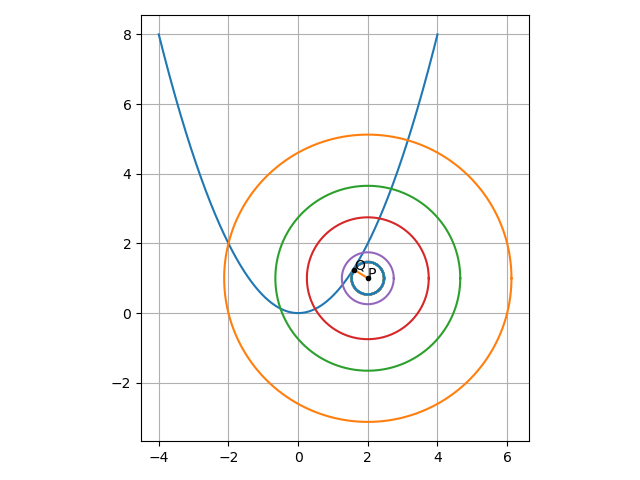
\includegraphics[width=\columnwidth]{12/6/5/27/conv/grad/figs/grad_pits.png}
        \caption{Gradient descent for a convex optimization problem.}
        \label{fig:12/6/5/27/conv/gradgd-pits}
    \end{figure}

\item
\label{12/6/5/3}
\iffalse
\documentclass[journal,12pt,twocolumn]{IEEEtran}
\usepackage{setspace}
\usepackage{gensymb}
\usepackage{xcolor}
\usepackage{caption}
\singlespacing
\usepackage{siunitx}
\usepackage[cmex10]{amsmath}
\usepackage{mathtools}
\usepackage{hyperref}
\usepackage{amsthm}
\usepackage{mathrsfs}
\usepackage{txfonts}
\usepackage{stfloats}
\usepackage{cite}
\usepackage{cases}
\usepackage{subfig}
\usepackage{longtable}
\usepackage{multirow}
\usepackage{enumitem}
\usepackage{bm}
\usepackage{mathtools}
\usepackage{listings}
\usepackage{tikz}
\usetikzlibrary{shapes,arrows,positioning}
\usepackage{circuitikz}
\renewcommand{\vec}[1]{\boldsymbol{\mathbf{#1}}}
\DeclareMathOperator*{\Res}{Res}
\renewcommand\thesection{\arabic{section}}
\renewcommand\thesubsection{\thesection.\arabic{subsection}}
\renewcommand\thesubsubsection{\thesubsection.\arabic{subsubsection}}

\renewcommand\thesectiondis{\arabic{section}}
\renewcommand\thesubsectiondis{\thesectiondis.\arabic{subsection}}
\renewcommand\thesubsubsectiondis{\thesubsectiondis.\arabic{subsubsection}}
\hyphenation{op-tical net-works semi-conduc-tor}

\lstset{
language=Python,
frame=single, 
breaklines=true,
columns=fullflexible
}
\begin{document}
\theoremstyle{definition}
\newtheorem{theorem}{Theorem}[section]
\newtheorem{problem}{Problem}
\newtheorem{proposition}{Proposition}[section]
\newtheorem{lemma}{Lemma}[section]
\newtheorem{corollary}[theorem]{Corollary}
\newtheorem{example}{Example}[section]
\newtheorem{definition}{Definition}[section]
\newcommand{\BEQA}{\begin{eqnarray}}
\newcommand{\EEQA}{\end{eqnarray}}
\newcommand{\define}{\stackrel{\triangle}{=}}
\newcommand{\myvec}[1]{\ensuremath{\begin{pmatrix}#1\end{pmatrix}}}
\newcommand{\mydet}[1]{\ensuremath{\begin{vmatrix}#1\end{vmatrix}}}
\bibliographystyle{IEEEtran}
\providecommand{\nCr}[2]{\,^{#1}C_{#2}} % nCr
\providecommand{\nPr}[2]{\,^{#1}P_{#2}} % nPr
\providecommand{\mbf}{\mathbf}
\providecommand{\pr}[1]{\ensuremath{\Pr\left(#1\right)}}
\providecommand{\qfunc}[1]{\ensuremath{Q\left(#1\right)}}
\providecommand{\sbrak}[1]{\ensuremath{{}\left[#1\right]}}
\providecommand{\lsbrak}[1]{\ensuremath{{}\left[#1\right.}}
\providecommand{\rsbrak}[1]{\ensuremath{{}\left.#1\right]}}
\providecommand{\brak}[1]{\ensuremath{\left(#1\right)}}
\providecommand{\lbrak}[1]{\ensuremath{\left(#1\right.}}
\providecommand{\rbrak}[1]{\ensuremath{\left.#1\right)}}
\providecommand{\cbrak}[1]{\ensuremath{\left\{#1\right\}}}
\providecommand{\lcbrak}[1]{\ensuremath{\left\{#1\right.}}
\providecommand{\rcbrak}[1]{\ensuremath{\left.#1\right\}}}
\theoremstyle{remark}
\newtheorem{rem}{Remark}
\newcommand{\sgn}{\mathop{\mathrm{sgn}}}
\newcommand{\rect}{\mathop{\mathrm{rect}}}
\newcommand{\sinc}{\mathop{\mathrm{sinc}}}
\providecommand{\abs}[1]{\left\vert#1\right\vert}
\providecommand{\res}[1]{\Res\displaylimits_{#1}} 
\providecommand{\norm}[1]{\left\Vert#1\right\Vert}
\providecommand{\mtx}[1]{\mathbf{#1}}
\providecommand{\mean}[1]{E\left[ #1 \right]}
\providecommand{\fourier}{\overset{\mathcal{F}}{ \rightleftharpoons}}
\providecommand{\ztrans}{\overset{\mathcal{Z}}{ \rightleftharpoons}}
\providecommand{\system}[1]{\overset{\mathcal{#1}}{ \longleftrightarrow}}
\newcommand{\solution}{\noindent \textbf{Solution: }}
\providecommand{\dec}[2]{\ensuremath{\overset{#1}{\underset{#2}{\gtrless}}}}
\let\StandardTheFigure\thefigure
\def\putbox#1#2#3{\makebox[0in][l]{\makebox[#1][l]{}\raisebox{\baselineskip}[0in][0in]{\raisebox{#2}[0in][0in]{#3}}}}
     \def\rightbox#1{\makebox[0in][r]{#1}}
     \def\centbox#1{\makebox[0in]{#1}}
     \def\topbox#1{\raisebox{-\baselineskip}[0in][0in]{#1}}
     \def\midbox#1{\raisebox{-0.5\baselineskip}[0in][0in]{#1}}

\vspace{3cm}
\title{Quadratic Programming Assignment}
\author{Gautam Singh}
\maketitle
\bigskip

\begin{abstract}
    This document contains the solution to a modification to Question 27 of 
    Exercise 5 in Chapter 6 of the class 12 NCERT textbook.
\end{abstract}

\begin{enumerate}
      \solution 
\fi
		We need to find
    \begin{align}
        \min_{\vec{x}} g\brak{\vec{x}} &= \norm{\vec{x}-\vec{P}}^2 \label{eq:12/6/5/27/conv/gradcost} \\
        \textrm{s.t. } h\brak{\vec{x}} &= \vec{x}^\top\vec{Vx} + 2\vec{u}^\top\vec{x} = 0 \label{eq:12/6/5/27/conv/gradconstr}
    \end{align}
    where
    \begin{align}
        \vec{V} = \myvec{1&0\\0&0},\ \vec{u} = \myvec{0\\-1}
    \end{align}

    We find the required minima using constrained gradient descent in 
    Fig. \ref{fig:12/6/5/27/conv/gradgd-pits}, plotted using Python.
    \begin{figure}[!ht]
        \centering
        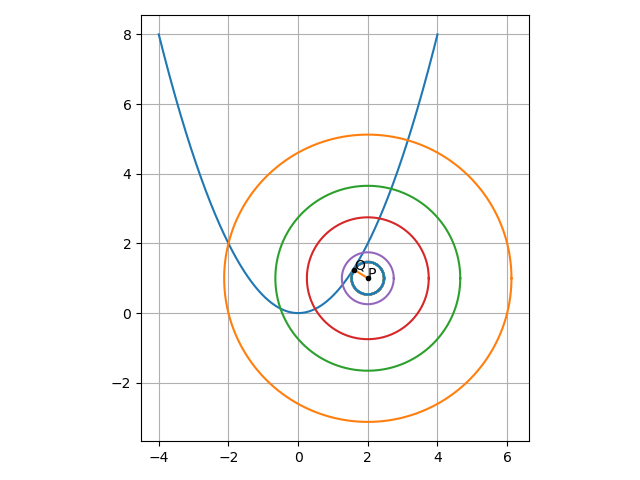
\includegraphics[width=\columnwidth]{12/6/5/27/conv/grad/figs/grad_pits.png}
        \caption{Gradient descent for a convex optimization problem.}
        \label{fig:12/6/5/27/conv/gradgd-pits}
    \end{figure}

\item
\label{12/6/5/4}
\iffalse
\documentclass[journal,12pt,twocolumn]{IEEEtran}
\usepackage{setspace}
\usepackage{gensymb}
\usepackage{xcolor}
\usepackage{caption}
\singlespacing
\usepackage{siunitx}
\usepackage[cmex10]{amsmath}
\usepackage{mathtools}
\usepackage{hyperref}
\usepackage{amsthm}
\usepackage{mathrsfs}
\usepackage{txfonts}
\usepackage{stfloats}
\usepackage{cite}
\usepackage{cases}
\usepackage{subfig}
\usepackage{longtable}
\usepackage{multirow}
\usepackage{enumitem}
\usepackage{bm}
\usepackage{mathtools}
\usepackage{listings}
\usepackage{tikz}
\usetikzlibrary{shapes,arrows,positioning}
\usepackage{circuitikz}
\renewcommand{\vec}[1]{\boldsymbol{\mathbf{#1}}}
\DeclareMathOperator*{\Res}{Res}
\renewcommand\thesection{\arabic{section}}
\renewcommand\thesubsection{\thesection.\arabic{subsection}}
\renewcommand\thesubsubsection{\thesubsection.\arabic{subsubsection}}

\renewcommand\thesectiondis{\arabic{section}}
\renewcommand\thesubsectiondis{\thesectiondis.\arabic{subsection}}
\renewcommand\thesubsubsectiondis{\thesubsectiondis.\arabic{subsubsection}}
\hyphenation{op-tical net-works semi-conduc-tor}

\lstset{
language=Python,
frame=single, 
breaklines=true,
columns=fullflexible
}
\begin{document}
\theoremstyle{definition}
\newtheorem{theorem}{Theorem}[section]
\newtheorem{problem}{Problem}
\newtheorem{proposition}{Proposition}[section]
\newtheorem{lemma}{Lemma}[section]
\newtheorem{corollary}[theorem]{Corollary}
\newtheorem{example}{Example}[section]
\newtheorem{definition}{Definition}[section]
\newcommand{\BEQA}{\begin{eqnarray}}
\newcommand{\EEQA}{\end{eqnarray}}
\newcommand{\define}{\stackrel{\triangle}{=}}
\newcommand{\myvec}[1]{\ensuremath{\begin{pmatrix}#1\end{pmatrix}}}
\newcommand{\mydet}[1]{\ensuremath{\begin{vmatrix}#1\end{vmatrix}}}
\bibliographystyle{IEEEtran}
\providecommand{\nCr}[2]{\,^{#1}C_{#2}} % nCr
\providecommand{\nPr}[2]{\,^{#1}P_{#2}} % nPr
\providecommand{\mbf}{\mathbf}
\providecommand{\pr}[1]{\ensuremath{\Pr\left(#1\right)}}
\providecommand{\qfunc}[1]{\ensuremath{Q\left(#1\right)}}
\providecommand{\sbrak}[1]{\ensuremath{{}\left[#1\right]}}
\providecommand{\lsbrak}[1]{\ensuremath{{}\left[#1\right.}}
\providecommand{\rsbrak}[1]{\ensuremath{{}\left.#1\right]}}
\providecommand{\brak}[1]{\ensuremath{\left(#1\right)}}
\providecommand{\lbrak}[1]{\ensuremath{\left(#1\right.}}
\providecommand{\rbrak}[1]{\ensuremath{\left.#1\right)}}
\providecommand{\cbrak}[1]{\ensuremath{\left\{#1\right\}}}
\providecommand{\lcbrak}[1]{\ensuremath{\left\{#1\right.}}
\providecommand{\rcbrak}[1]{\ensuremath{\left.#1\right\}}}
\theoremstyle{remark}
\newtheorem{rem}{Remark}
\newcommand{\sgn}{\mathop{\mathrm{sgn}}}
\newcommand{\rect}{\mathop{\mathrm{rect}}}
\newcommand{\sinc}{\mathop{\mathrm{sinc}}}
\providecommand{\abs}[1]{\left\vert#1\right\vert}
\providecommand{\res}[1]{\Res\displaylimits_{#1}} 
\providecommand{\norm}[1]{\left\Vert#1\right\Vert}
\providecommand{\mtx}[1]{\mathbf{#1}}
\providecommand{\mean}[1]{E\left[ #1 \right]}
\providecommand{\fourier}{\overset{\mathcal{F}}{ \rightleftharpoons}}
\providecommand{\ztrans}{\overset{\mathcal{Z}}{ \rightleftharpoons}}
\providecommand{\system}[1]{\overset{\mathcal{#1}}{ \longleftrightarrow}}
\newcommand{\solution}{\noindent \textbf{Solution: }}
\providecommand{\dec}[2]{\ensuremath{\overset{#1}{\underset{#2}{\gtrless}}}}
\let\StandardTheFigure\thefigure
\def\putbox#1#2#3{\makebox[0in][l]{\makebox[#1][l]{}\raisebox{\baselineskip}[0in][0in]{\raisebox{#2}[0in][0in]{#3}}}}
     \def\rightbox#1{\makebox[0in][r]{#1}}
     \def\centbox#1{\makebox[0in]{#1}}
     \def\topbox#1{\raisebox{-\baselineskip}[0in][0in]{#1}}
     \def\midbox#1{\raisebox{-0.5\baselineskip}[0in][0in]{#1}}

\vspace{3cm}
\title{Quadratic Programming Assignment}
\author{Gautam Singh}
\maketitle
\bigskip

\begin{abstract}
    This document contains the solution to a modification to Question 27 of 
    Exercise 5 in Chapter 6 of the class 12 NCERT textbook.
\end{abstract}

\begin{enumerate}
      \solution 
\fi
		We need to find
    \begin{align}
        \min_{\vec{x}} g\brak{\vec{x}} &= \norm{\vec{x}-\vec{P}}^2 \label{eq:12/6/5/27/conv/gradcost} \\
        \textrm{s.t. } h\brak{\vec{x}} &= \vec{x}^\top\vec{Vx} + 2\vec{u}^\top\vec{x} = 0 \label{eq:12/6/5/27/conv/gradconstr}
    \end{align}
    where
    \begin{align}
        \vec{V} = \myvec{1&0\\0&0},\ \vec{u} = \myvec{0\\-1}
    \end{align}

    We find the required minima using constrained gradient descent in 
    Fig. \ref{fig:12/6/5/27/conv/gradgd-pits}, plotted using Python.
    \begin{figure}[!ht]
        \centering
        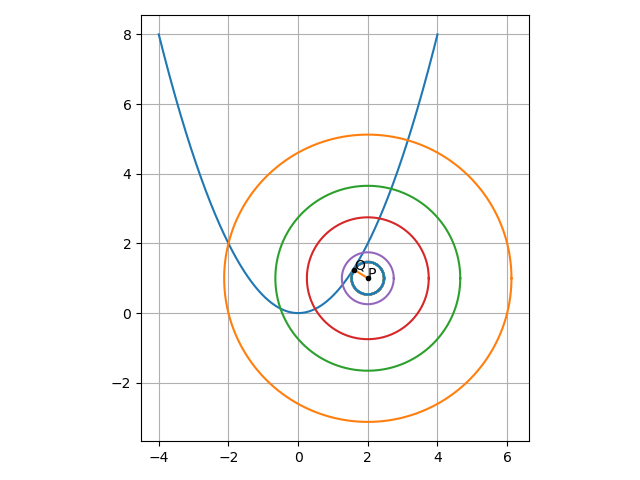
\includegraphics[width=\columnwidth]{12/6/5/27/conv/grad/figs/grad_pits.png}
        \caption{Gradient descent for a convex optimization problem.}
        \label{fig:12/6/5/27/conv/gradgd-pits}
    \end{figure}

\item
\label{12/6/5/5}
\iffalse
\documentclass[journal,12pt,twocolumn]{IEEEtran}
\usepackage{setspace}
\usepackage{gensymb}
\usepackage{xcolor}
\usepackage{caption}
\singlespacing
\usepackage{siunitx}
\usepackage[cmex10]{amsmath}
\usepackage{mathtools}
\usepackage{hyperref}
\usepackage{amsthm}
\usepackage{mathrsfs}
\usepackage{txfonts}
\usepackage{stfloats}
\usepackage{cite}
\usepackage{cases}
\usepackage{subfig}
\usepackage{longtable}
\usepackage{multirow}
\usepackage{enumitem}
\usepackage{bm}
\usepackage{mathtools}
\usepackage{listings}
\usepackage{tikz}
\usetikzlibrary{shapes,arrows,positioning}
\usepackage{circuitikz}
\renewcommand{\vec}[1]{\boldsymbol{\mathbf{#1}}}
\DeclareMathOperator*{\Res}{Res}
\renewcommand\thesection{\arabic{section}}
\renewcommand\thesubsection{\thesection.\arabic{subsection}}
\renewcommand\thesubsubsection{\thesubsection.\arabic{subsubsection}}

\renewcommand\thesectiondis{\arabic{section}}
\renewcommand\thesubsectiondis{\thesectiondis.\arabic{subsection}}
\renewcommand\thesubsubsectiondis{\thesubsectiondis.\arabic{subsubsection}}
\hyphenation{op-tical net-works semi-conduc-tor}

\lstset{
language=Python,
frame=single, 
breaklines=true,
columns=fullflexible
}
\begin{document}
\theoremstyle{definition}
\newtheorem{theorem}{Theorem}[section]
\newtheorem{problem}{Problem}
\newtheorem{proposition}{Proposition}[section]
\newtheorem{lemma}{Lemma}[section]
\newtheorem{corollary}[theorem]{Corollary}
\newtheorem{example}{Example}[section]
\newtheorem{definition}{Definition}[section]
\newcommand{\BEQA}{\begin{eqnarray}}
\newcommand{\EEQA}{\end{eqnarray}}
\newcommand{\define}{\stackrel{\triangle}{=}}
\newcommand{\myvec}[1]{\ensuremath{\begin{pmatrix}#1\end{pmatrix}}}
\newcommand{\mydet}[1]{\ensuremath{\begin{vmatrix}#1\end{vmatrix}}}
\bibliographystyle{IEEEtran}
\providecommand{\nCr}[2]{\,^{#1}C_{#2}} % nCr
\providecommand{\nPr}[2]{\,^{#1}P_{#2}} % nPr
\providecommand{\mbf}{\mathbf}
\providecommand{\pr}[1]{\ensuremath{\Pr\left(#1\right)}}
\providecommand{\qfunc}[1]{\ensuremath{Q\left(#1\right)}}
\providecommand{\sbrak}[1]{\ensuremath{{}\left[#1\right]}}
\providecommand{\lsbrak}[1]{\ensuremath{{}\left[#1\right.}}
\providecommand{\rsbrak}[1]{\ensuremath{{}\left.#1\right]}}
\providecommand{\brak}[1]{\ensuremath{\left(#1\right)}}
\providecommand{\lbrak}[1]{\ensuremath{\left(#1\right.}}
\providecommand{\rbrak}[1]{\ensuremath{\left.#1\right)}}
\providecommand{\cbrak}[1]{\ensuremath{\left\{#1\right\}}}
\providecommand{\lcbrak}[1]{\ensuremath{\left\{#1\right.}}
\providecommand{\rcbrak}[1]{\ensuremath{\left.#1\right\}}}
\theoremstyle{remark}
\newtheorem{rem}{Remark}
\newcommand{\sgn}{\mathop{\mathrm{sgn}}}
\newcommand{\rect}{\mathop{\mathrm{rect}}}
\newcommand{\sinc}{\mathop{\mathrm{sinc}}}
\providecommand{\abs}[1]{\left\vert#1\right\vert}
\providecommand{\res}[1]{\Res\displaylimits_{#1}} 
\providecommand{\norm}[1]{\left\Vert#1\right\Vert}
\providecommand{\mtx}[1]{\mathbf{#1}}
\providecommand{\mean}[1]{E\left[ #1 \right]}
\providecommand{\fourier}{\overset{\mathcal{F}}{ \rightleftharpoons}}
\providecommand{\ztrans}{\overset{\mathcal{Z}}{ \rightleftharpoons}}
\providecommand{\system}[1]{\overset{\mathcal{#1}}{ \longleftrightarrow}}
\newcommand{\solution}{\noindent \textbf{Solution: }}
\providecommand{\dec}[2]{\ensuremath{\overset{#1}{\underset{#2}{\gtrless}}}}
\let\StandardTheFigure\thefigure
\def\putbox#1#2#3{\makebox[0in][l]{\makebox[#1][l]{}\raisebox{\baselineskip}[0in][0in]{\raisebox{#2}[0in][0in]{#3}}}}
     \def\rightbox#1{\makebox[0in][r]{#1}}
     \def\centbox#1{\makebox[0in]{#1}}
     \def\topbox#1{\raisebox{-\baselineskip}[0in][0in]{#1}}
     \def\midbox#1{\raisebox{-0.5\baselineskip}[0in][0in]{#1}}

\vspace{3cm}
\title{Quadratic Programming Assignment}
\author{Gautam Singh}
\maketitle
\bigskip

\begin{abstract}
    This document contains the solution to a modification to Question 27 of 
    Exercise 5 in Chapter 6 of the class 12 NCERT textbook.
\end{abstract}

\begin{enumerate}
      \solution 
\fi
		We need to find
    \begin{align}
        \min_{\vec{x}} g\brak{\vec{x}} &= \norm{\vec{x}-\vec{P}}^2 \label{eq:12/6/5/27/conv/gradcost} \\
        \textrm{s.t. } h\brak{\vec{x}} &= \vec{x}^\top\vec{Vx} + 2\vec{u}^\top\vec{x} = 0 \label{eq:12/6/5/27/conv/gradconstr}
    \end{align}
    where
    \begin{align}
        \vec{V} = \myvec{1&0\\0&0},\ \vec{u} = \myvec{0\\-1}
    \end{align}

    We find the required minima using constrained gradient descent in 
    Fig. \ref{fig:12/6/5/27/conv/gradgd-pits}, plotted using Python.
    \begin{figure}[!ht]
        \centering
        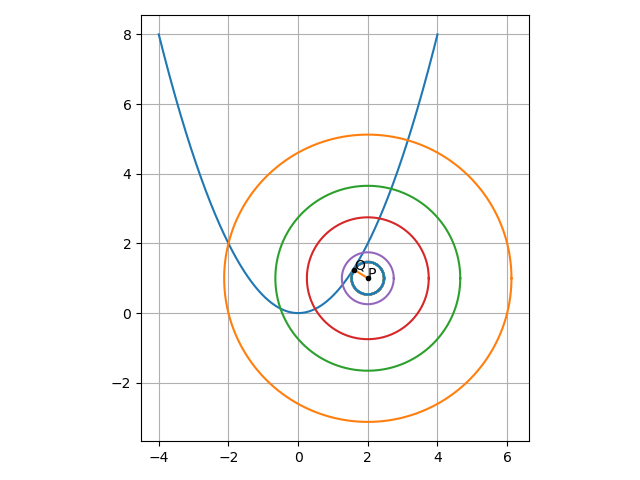
\includegraphics[width=\columnwidth]{12/6/5/27/conv/grad/figs/grad_pits.png}
        \caption{Gradient descent for a convex optimization problem.}
        \label{fig:12/6/5/27/conv/gradgd-pits}
    \end{figure}

\fi
\item
\label{12/6/5/6}
\iffalse
\documentclass[journal,10pt,twocolumn]{article}
\usepackage{graphicx, float}
\usepackage[margin=0.5in]{geometry}
\usepackage{amsmath, bm}
\usepackage{array}
\usepackage{booktabs}
\usepackage[utf8]{inputenc}
\usepackage{amsfonts}
\usepackage{amssymb}
\usepackage{graphicx}
\usepackage{multicol}
\usepackage{tabularx}
\usepackage{hyperref}
\usepackage{mathtools}
\DeclareUnicodeCharacter{2212}{-}
\providecommand{\norm}[1]{\left\lVert#1\right\rVert}
\providecommand{\abs}[1]{\left\vert#1\right\vert}
\let\vec\mathbf
\newcommand{\myvec}[1]{\ensuremath{\begin{pmatrix}#1\end{pmatrix}}}
\newcommand{\mydet}[1]{\ensuremath{\begin{vmatrix}#1\end{vmatrix}}}
\providecommand{\brak}[1]{\ensuremath{\left(#1\right)}}
\providecommand{\lbrak}[1]{\ensuremath{\left(#1\right.}}
\providecommand{\rbrak}[1]{\ensuremath{\left.#1\right)}}
\providecommand{\sbrak}[1]{\ensuremath{{}\left[#1\right]}}
%\providecommand{\norm}[1]{\left\lVert#1\right\rVert}
%\providecommand{\sbrak}[1]{\ensuremath{{}\left[#1\right]}}
%\providecommand{\lsbrak}[1]{\ensuremath{{}\left[#1\right.}}
%\providecommand{\rsbrak}[1]{\ensuremath{{}\left.#1\right]}}
%\providecommand{\brak}[1]{\ensuremath{\left(#1\right)}}
%\providecommand{\lbrak}[1]{\ensuremath{\left(#1\right.}}
%\providecommand{\rbrak}[1]{\ensuremath{\left.#1\right)}}
%\providecommand{\cbrak}[1]{\ensuremath{\left\{#1\right\}}}
%\providecommand{\lcbrak}[1]{\ensuremath{\left\{#1\right.}}
%\providecommand{\rcbrak}[1]{\ensuremath{\left.#1\right\}}}
%\newcommand{\myvec}[1]{\ensuremath{\begin{pmatrix}#1\end{pmatrix}}}
%\let\vec\mathbf

\title{\textbf{Optimization-Basic Assignment}}
\author{Namrath Pinnamaneni \hspace{9cm} FWC22042}
\date{September 2022}

\begin{document}

\maketitle
\paragraph{\textit{Problem Statement} -
\fi
Find the maximum profit that a company can make if the profit function is given by  
\begin{align}
f(x) = 41-72x+18x^2
\end{align}
\\
\solution
\iffalse
A function f(x) is said to be convex if following inequality is true for $\lambda \in [0,1] :$  \label{opt/2/1/a/lemma1}
\begin{align}
    \lambda f(x_1) + (1-\lambda)f(x_2) \geq f(\lambda x_1 + (1-\lambda)x_2)
    \label{eq:12/6/5/62}
\end{align}
\fi
Considering
\begin{align}
    &\lambda\brak{41-72x_1-18x_1^2} + (1-\lambda)\brak{41-72x_2-18x_2^2} \geq \\
    &41-72\brak{\lambda x_1 + (1-\lambda)x_2} - 18\brak{\lambda x_1 + (1-\lambda)x_2}^2,
\end{align}
we obtain
\begin{align}
        18x_1^2\brak{{\lambda^2-\lambda}}+18x_2^2\brak{{\lambda^2-\lambda}}+36x_1x_2\brak{{\lambda^2-\lambda}} &\geq 0 \\
        x_1^2\brak{{\lambda^2-\lambda}}+x_2^2\brak{{\lambda^2-\lambda}}+2x_1x_2\brak{{\lambda^2-\lambda}} &\geq 0 \\
        -\lambda\brak{1-\lambda}\brak{x_1-x_2}^2 &\geq 0 \\
        \implies \lambda\brak{1-\lambda}\brak{x_1-x_2}^2 &\leq 0 \label{eq:12/6/5/67}
\end{align}
which is 
 false for all $\lambda\in(0,1)$. Hence the given function $f(x)$ is concave.
 \iffalse
 For a general quadratic equation
\begin{align}
    f(x)=ax^2+bx+c
\end{align}
\fi
    Using the gradient ascent method,
\begin{align}
    x_n=x_{n-1}+\mu\frac{df(x)}{dx} \label{eq:12/6/5/69}
    \end{align}
    Since
    \begin{align}
    \frac{df(x)}{dx}=-72-36x, \label{eq:12/6/5/610}
\end{align}
substituting \eqref{eq:12/6/5/610} in \eqref{eq:12/6/5/69}, 
\begin{align}
    x_n=x_{n-1}+\mu(-72-36x_{n-1})\label{eq:12/6/5/611}
\end{align}
Choosing
\begin{align}
	x_0 &= 1, \alpha = 0.001,  precision = 0.00000001, 
\\
	f_{max}  &\approx 113,
	x_{max}  \approx -2.0,
\end{align}
which is verified in Fig. 
		\ref{fig:12/6/5/6}.
	\begin{figure}[!ht]
		\centering
		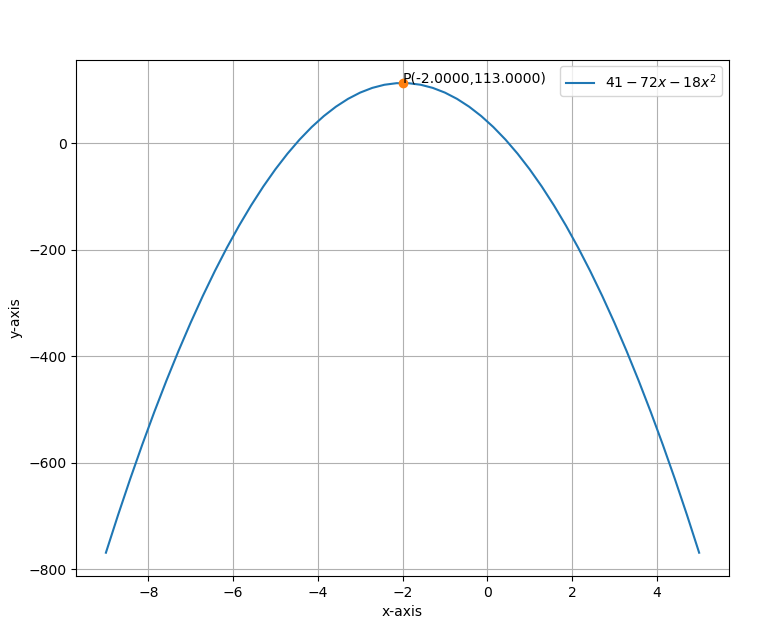
\includegraphics[width=\columnwidth]{12/6/5/6/figs/opt_basic.png}
		\caption{}
		\label{fig:12/6/5/6}
  	\end{figure}
\iffalse
\includegraphics[width=1\columnwidth]{opt_basic.png}
\centering \text{Graph of f(x) = $41-72x+18x^2$}

\end{document}
\fi

\item
\label{12/6/5/7}
\iffalse
\documentclass[journal,10pt,twocolumn]{article}
\usepackage{graphicx, float}
\usepackage[margin=0.5in]{geometry}
\usepackage{amsmath, bm}
\usepackage{array}
\usepackage{booktabs}

\providecommand{\norm}[1]{\left\lVert#1\right\rVert}
\let\vec\mathbf
\newcommand{\myvec}[1]{\ensuremath{\begin{pmatrix}#1\end{pmatrix}}}
\newcommand{\mydet}[1]{\ensuremath{\begin{vmatrix}#1\end{vmatrix}}}

\title{\textbf{Optimization Assignment}}
\author{Pallavarapu Sravan kumar}
\date{October 2022}

\begin{document}

\maketitle
\paragraph{\textit{\large Problem Statement} -
\fi
Find both the maximum value and the minimum value of 
\begin{align}
    f(x) &= 3x^4-8x^3+12x^2-48x+25=0 &  x \in (0,3)
\end{align}
\solution
	\begin{figure}[!ht]
		\centering
		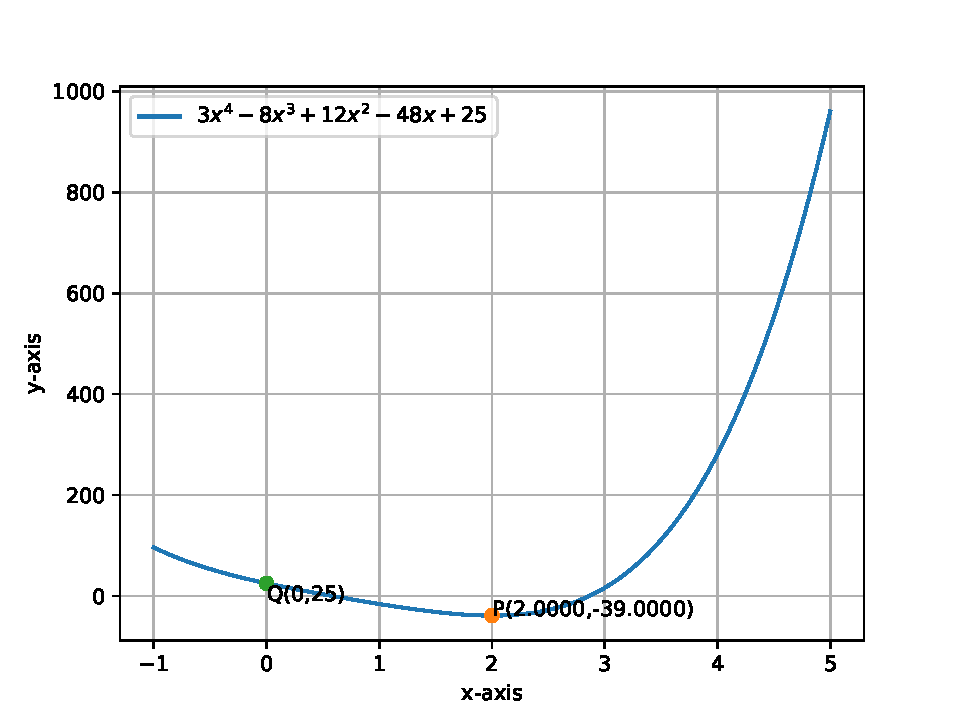
\includegraphics[width=\columnwidth]{12/6/5/7/figs/opt2.pdf}
		\caption{}
		\label{fig:12/6/5/7}
  	\end{figure}
	\iffalse
\section*{\large Figure:}
\begin{figure}[H]
\centering
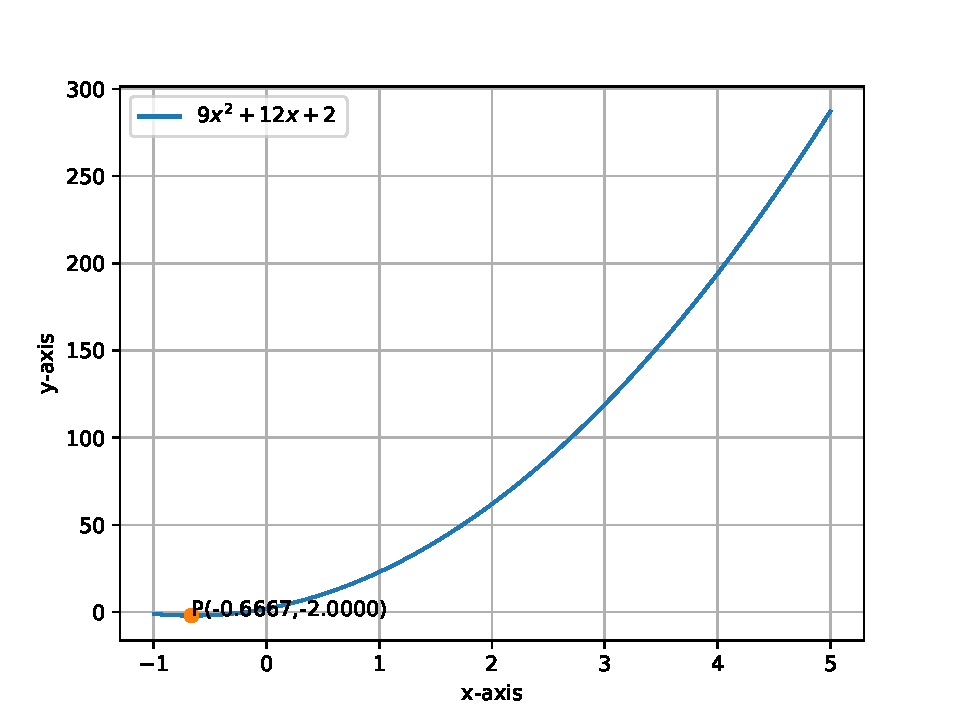
\includegraphics[width=1\columnwidth]{opt2.pdf}
\caption{Graph of f(x)}
\end{figure}



\section*{Solution:}

Given:
\begin{align}
    f(x) &= 3x^4-8x^3+12x^2-48x+25=0 &  x \in (0,3)
\end{align}
\fi
\begin{align}
    \frac{df(x)}{dx} &= 12x^3-24x^2+24x-48
\end{align}
		The minimum can be found using
\begin{align}
        x_{n+1} &= x_n - \alpha \frac{df(x)}{dx}
	\\
          &= x_n - \alpha (12x_n^3-24x_n^2+24x_n-48)
\end{align}
where 
\begin{enumerate}
\item $\alpha$ = 0.001
\item $x_{n+1}$ is current value
\item $x_{n}$ is previous value
\item precession = 0.00000001
\item maximum iterations = 100000000
\end{enumerate}
as
\begin{align}
 	f_{min}= -39\\
 	x_{min}= 2
    \end{align}
    \iffalse
    \item
For maximum, the 
 Critical point is given by
    \begin{align}
       \frac{df(x)}{dx} &= 0 \\
        \implies x &= 2
    \end{align}
    
    and,end points are $x=0$ and $x=3$ .Using table1
    \begin{table}[htbp]
 \begin{center}
    \begin{tabular}{|l|c|c|c|c|c|c} \hline \textbf{x}
  & \textbf{f(x)} \\
 \hline
0 &25\\ \hline
2&-39 \\ \hline
3 &16  \\ \hline	
\end{tabular}   
\end{center}
\caption{Value of f(x)}
\end{table}

 \begin{align}
        \boxed{\text{Maxima} = 25}\\
        \boxed{\text{Maxima Point} = 0}
    \end{align}
   
\end{document}
\fi

\item
\label{12/6/5/8}
\iffalse
\documentclass[journal,10pt,twocolumn]{article}
\usepackage{graphicx, float}
\usepackage[margin=0.5in]{geometry}
\usepackage{amsmath, bm}
\usepackage{array}
\usepackage{booktabs}
\usepackage{mathtools}

\providecommand{\norm}[1]{\left\lVert#1\right\rVert}
\let\vec\mathbf
\newcommand{\myvec}[1]{\ensuremath{\begin{pmatrix}#1\end{pmatrix}}}
\newcommand{\mydet}[1]{\ensuremath{\begin{vmatrix}#1\end{vmatrix}}}

\title{\textbf{Optimization Assignment}}
\author{Maddu Dinesh}
\date{September 2022}

\begin{document}

\maketitle
\paragraph{\textit{Problem Statement} -
\fi
At what points in the interval (0,2$\pi$) does the function $\sin2x$ attain its maximum value.
\\
\solution
	\begin{figure}[!ht]
		\centering
		\includegraphics[width=\columnwidth]{12/6/5/8/figs/a.png}
		\caption{}
		\label{fig:12/6/5/8}
  	\end{figure}
\iffalse
\section*{\large Figure}

\begin{figure}[H]
\centering
\includegraphics[width=1\columnwidth]{a.png}
\caption{Graph of f(x)}
\label{fig:triangle}
\end{figure}
\section*{\large Solution}

	
    \subsection*{\normalsize Gradient descent}
\fi    
  Since  
    \begin{align}
	\label{eq:12/6/5/8vol_varx}
	    f(x) &= \sin2x,
	    \\
	    f'(x) &= 2\cos2x
	\end{align}
\iffalse
we have to attain the maximum value of sin2x in the interval [0,2$\pi$]. This can be seen in Figure f(x).
\fi
Using gradient ascent, 
\begin{align}
	x_{n+1} &= x_n + \alpha \nabla f(x_n) \\
&=x_n+\alpha(2\cos2x)
\end{align}
Choosing
\begin{align}
	x_0&=0.5,\alpha=0.001, precision = 0.00000001, 
	\\
	f_{max} &= 1.0000,
 	x_{max}= 0.7854.
    \end{align}
   
    

    





 







\iffalse
\item
\label{12/6/5/9}
%\iffalse
\documentclass[journal,12pt,twocolumn]{IEEEtran}
\usepackage{setspace}
\usepackage{gensymb}
\usepackage{xcolor}
\usepackage{caption}
\singlespacing
\usepackage{siunitx}
\usepackage[cmex10]{amsmath}
\usepackage{mathtools}
\usepackage{hyperref}
\usepackage{amsthm}
\usepackage{mathrsfs}
\usepackage{txfonts}
\usepackage{stfloats}
\usepackage{cite}
\usepackage{cases}
\usepackage{subfig}
\usepackage{longtable}
\usepackage{multirow}
\usepackage{enumitem}
\usepackage{bm}
\usepackage{mathtools}
\usepackage{listings}
\usepackage{tikz}
\usetikzlibrary{shapes,arrows,positioning}
\usepackage{circuitikz}
\renewcommand{\vec}[1]{\boldsymbol{\mathbf{#1}}}
\DeclareMathOperator*{\Res}{Res}
\renewcommand\thesection{\arabic{section}}
\renewcommand\thesubsection{\thesection.\arabic{subsection}}
\renewcommand\thesubsubsection{\thesubsection.\arabic{subsubsection}}

\renewcommand\thesectiondis{\arabic{section}}
\renewcommand\thesubsectiondis{\thesectiondis.\arabic{subsection}}
\renewcommand\thesubsubsectiondis{\thesubsectiondis.\arabic{subsubsection}}
\hyphenation{op-tical net-works semi-conduc-tor}

\lstset{
language=Python,
frame=single, 
breaklines=true,
columns=fullflexible
}
\begin{document}
\theoremstyle{definition}
\newtheorem{theorem}{Theorem}[section]
\newtheorem{problem}{Problem}
\newtheorem{proposition}{Proposition}[section]
\newtheorem{lemma}{Lemma}[section]
\newtheorem{corollary}[theorem]{Corollary}
\newtheorem{example}{Example}[section]
\newtheorem{definition}{Definition}[section]
\newcommand{\BEQA}{\begin{eqnarray}}
\newcommand{\EEQA}{\end{eqnarray}}
\newcommand{\define}{\stackrel{\triangle}{=}}
\newcommand{\myvec}[1]{\ensuremath{\begin{pmatrix}#1\end{pmatrix}}}
\newcommand{\mydet}[1]{\ensuremath{\begin{vmatrix}#1\end{vmatrix}}}
\bibliographystyle{IEEEtran}
\providecommand{\nCr}[2]{\,^{#1}C_{#2}} % nCr
\providecommand{\nPr}[2]{\,^{#1}P_{#2}} % nPr
\providecommand{\mbf}{\mathbf}
\providecommand{\pr}[1]{\ensuremath{\Pr\left(#1\right)}}
\providecommand{\qfunc}[1]{\ensuremath{Q\left(#1\right)}}
\providecommand{\sbrak}[1]{\ensuremath{{}\left[#1\right]}}
\providecommand{\lsbrak}[1]{\ensuremath{{}\left[#1\right.}}
\providecommand{\rsbrak}[1]{\ensuremath{{}\left.#1\right]}}
\providecommand{\brak}[1]{\ensuremath{\left(#1\right)}}
\providecommand{\lbrak}[1]{\ensuremath{\left(#1\right.}}
\providecommand{\rbrak}[1]{\ensuremath{\left.#1\right)}}
\providecommand{\cbrak}[1]{\ensuremath{\left\{#1\right\}}}
\providecommand{\lcbrak}[1]{\ensuremath{\left\{#1\right.}}
\providecommand{\rcbrak}[1]{\ensuremath{\left.#1\right\}}}
\theoremstyle{remark}
\newtheorem{rem}{Remark}
\newcommand{\sgn}{\mathop{\mathrm{sgn}}}
\newcommand{\rect}{\mathop{\mathrm{rect}}}
\newcommand{\sinc}{\mathop{\mathrm{sinc}}}
\providecommand{\abs}[1]{\left\vert#1\right\vert}
\providecommand{\res}[1]{\Res\displaylimits_{#1}} 
\providecommand{\norm}[1]{\left\Vert#1\right\Vert}
\providecommand{\mtx}[1]{\mathbf{#1}}
\providecommand{\mean}[1]{E\left[ #1 \right]}
\providecommand{\fourier}{\overset{\mathcal{F}}{ \rightleftharpoons}}
\providecommand{\ztrans}{\overset{\mathcal{Z}}{ \rightleftharpoons}}
\providecommand{\system}[1]{\overset{\mathcal{#1}}{ \longleftrightarrow}}
\newcommand{\solution}{\noindent \textbf{Solution: }}
\providecommand{\dec}[2]{\ensuremath{\overset{#1}{\underset{#2}{\gtrless}}}}
\let\StandardTheFigure\thefigure
\def\putbox#1#2#3{\makebox[0in][l]{\makebox[#1][l]{}\raisebox{\baselineskip}[0in][0in]{\raisebox{#2}[0in][0in]{#3}}}}
     \def\rightbox#1{\makebox[0in][r]{#1}}
     \def\centbox#1{\makebox[0in]{#1}}
     \def\topbox#1{\raisebox{-\baselineskip}[0in][0in]{#1}}
     \def\midbox#1{\raisebox{-0.5\baselineskip}[0in][0in]{#1}}

\vspace{3cm}
\title{Quadratic Programming Assignment}
\author{Gautam Singh}
\maketitle
\bigskip

\begin{abstract}
    This document contains the solution to a modification to Question 27 of 
    Exercise 5 in Chapter 6 of the class 12 NCERT textbook.
\end{abstract}

\begin{enumerate}
      \solution 
\fi
		We need to find
    \begin{align}
        \min_{\vec{x}} g\brak{\vec{x}} &= \norm{\vec{x}-\vec{P}}^2 \label{eq:12/6/5/27/conv/gradcost} \\
        \textrm{s.t. } h\brak{\vec{x}} &= \vec{x}^\top\vec{Vx} + 2\vec{u}^\top\vec{x} = 0 \label{eq:12/6/5/27/conv/gradconstr}
    \end{align}
    where
    \begin{align}
        \vec{V} = \myvec{1&0\\0&0},\ \vec{u} = \myvec{0\\-1}
    \end{align}

    We find the required minima using constrained gradient descent in 
    Fig. \ref{fig:12/6/5/27/conv/gradgd-pits}, plotted using Python.
    \begin{figure}[!ht]
        \centering
        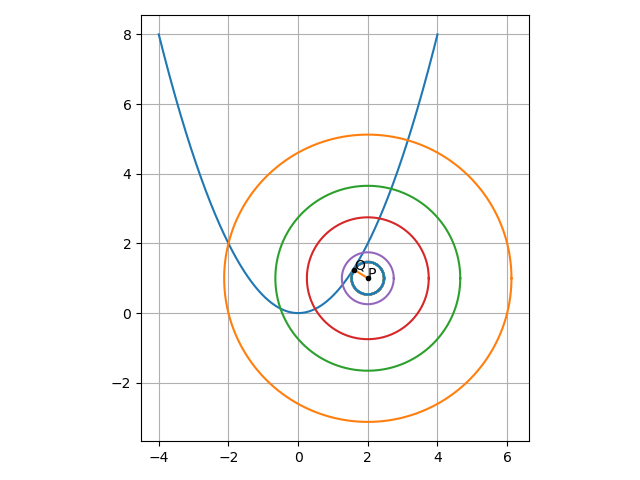
\includegraphics[width=\columnwidth]{12/6/5/27/conv/grad/figs/grad_pits.png}
        \caption{Gradient descent for a convex optimization problem.}
        \label{fig:12/6/5/27/conv/gradgd-pits}
    \end{figure}

\fi
\item
\label{12/6/5/10}
\iffalse
\documentclass[journal,10pt,twocolumn]{article}
\usepackage{graphicx, float}
\usepackage[margin=0.5in]{geometry}
\usepackage{amsmath, bm}
\usepackage{array}
\usepackage{booktabs}
\usepackage[utf8]{inputenc}
\usepackage{amsfonts}
\usepackage{amssymb}
\usepackage{graphicx}
\usepackage{multicol}
\usepackage{tabularx}
\usepackage{hyperref}
\usepackage{mathtools}
\DeclareUnicodeCharacter{2212}{-}
\providecommand{\norm}[1]{\left\lVert#1\right\rVert}
\providecommand{\abs}[1]{\left\vert#1\right\vert}
\let\vec\mathbf
\newcommand{\myvec}[1]{\ensuremath{\begin{pmatrix}#1\end{pmatrix}}}
\newcommand{\mydet}[1]{\ensuremath{\begin{vmatrix}#1\end{vmatrix}}}
\providecommand{\brak}[1]{\ensuremath{\left(#1\right)}}
\providecommand{\lbrak}[1]{\ensuremath{\left(#1\right.}}
\providecommand{\rbrak}[1]{\ensuremath{\left.#1\right)}}
\providecommand{\sbrak}[1]{\ensuremath{{}\left[#1\right]}}
%\providecommand{\norm}[1]{\left\lVert#1\right\rVert}
%\providecommand{\sbrak}[1]{\ensuremath{{}\left[#1\right]}}
%\providecommand{\lsbrak}[1]{\ensuremath{{}\left[#1\right.}}
%\providecommand{\rsbrak}[1]{\ensuremath{{}\left.#1\right]}}
%\providecommand{\brak}[1]{\ensuremath{\left(#1\right)}}
%\providecommand{\lbrak}[1]{\ensuremath{\left(#1\right.}}
%\providecommand{\rbrak}[1]{\ensuremath{\left.#1\right)}}
%\providecommand{\cbrak}[1]{\ensuremath{\left\{#1\right\}}}
%\providecommand{\lcbrak}[1]{\ensuremath{\left\{#1\right.}}
%\providecommand{\rcbrak}[1]{\ensuremath{\left.#1\right\}}}
%\newcommand{\myvec}[1]{\ensuremath{\begin{pmatrix}#1\end{pmatrix}}}
%\let\vec\mathbf

\title{\textbf{Optimization-Basic Assignment}}
\author{V.Meghana \hspace{9cm} FWC22045}
\date{October 2022}

\begin{document}

\maketitle
\paragraph{\textit{Problem Statement} -
\fi
Find the maximum value of $2x^3 – 24x + 107$ in the interval [1, 3]. Find the maximum value of the same function in [–3, –1].
\\
\solution
\iffalse
\section*{\large Solution}
\fi
    Using gradient ascent method,
\begin{align}
    x_n=x_{n-1}+\mu\frac{df(x)}{dx} \label{eq:12/6/5/109}
    \end{align}
    where
    \begin{align}
    \frac{df(x)}{dx}=6x^2-24 \label{eq:12/6/5/1010}
\end{align}
yielding
\begin{align}
    x_n=x_{n-1}+\mu(6x^2-24_{n-1})\label{eq:12/6/5/1011}
\end{align}
Choosing
\begin{align}
	x_0 &= 1, \mu = 0.001 \text{ and precision} = 0.00000001, 
	\\
	f_{max} &  \approx 139,
x_{max}   \approx -2.0
\end{align}
	\begin{figure}[!ht]
		\centering
		\includegraphics[width=\columnwidth]{12/6/5/10/figs/opt_basic.png}
		\caption{}
		\label{fig:12/6/5/10}
  	\end{figure}
\iffalse
\begin{align}
\end{align}
\end{enumerate}

\includegraphics[width=1\columnwidth]{opt_basic.png}
\centering \text{Graph of f(x) = $2x^3-24x+107$}

\end{document}
\fi

\item
\label{12/6/5/11}
\iffalse
\documentclass[10pt,twocolumn]{article}
\usepackage{graphicx}
\usepackage[margin=0.5in]{geometry}
\usepackage[cmex10]{amsmath}
\usepackage{array}
\usepackage{booktabs}
\usepackage{mathtools}
\title{\textbf{Optimization}}
\author{Vemulapalli Bavya Sri}
\date{October 2022}


\providecommand{\norm}[1]{\lVert#1\rVert}
\providecommand{\abs}[1]{\vert#1\vert}
\let\vec\mathbf
\newcommand{\myvec}[1]{\ensuremath{\begin{pmatrix}#1\end{pmatrix}}}
\newcommand{\mydet}[1]{\ensuremath{\begin{vmatrix}#1\end{vmatrix}}}
\providecommand{\brak}[1]{\ensuremath{\left(#1\right)}}
\providecommand{\lbrak}[1]{\ensuremath{\left(#1\right.}}
\providecommand{\rbrak}[1]{\ensuremath{\left.#1\right)}}
\providecommand{\sbrak}[1]{\ensuremath{{}\left[#1\right]}}

\begin{document}

\maketitle
\paragraph{\textit{Problem Statement} -
\fi
It is given that at x=1, the function
$x^4-62x^2+ax+9$ attains its maximum value, on the interval [0,2]. Find the value of a. 
\\
\solution
\iffalse
\section{Solution}
\begin{flushleft}
Given function is,\\
\end{flushleft}
\begin{align}
\label{eqn:1}
    f(x)=x^4-62x^2+ax+9
\end{align}
\subsection{Calculation of Maxima using normal differentiation}
\begin{flushleft}
	\fi
Differentiating the given function,
\begin{align}
\nabla f(x) = 4x^3-124x+a
\end{align}
Since $f$ attains its maximum value on the interval [0,2] at $x=1$,
\begin{align}
\nabla f(1) =0
\implies a=120
\end{align}
\iffalse
\begin{flushleft}
\subsection{Calculation of Maxima using gradient ascent algorithm}
\end{flushleft}
\begin{flushleft}
Maxima of the above equation (1), can be calculated from the following expression,\\
To find,
\end{flushleft}
\begin{align}
\max_{x} f(x)
\end{align}  
\fi
Using gradient descent,
    \begin{align}
	    x_{n+1}&= x_n + \alpha \nabla f(x_n)
	    \\
	    &= x_n + \alpha \brak{4x_n^3-124x_n+120}
    \end{align}
    and choosing
\begin{align}
	x_0&=0.5,\alpha=0.001 \text{ and precision} = 0.00000001, 
	\\
	f_{max} &= 68,
        x_{max} = 1
\end{align}
	\begin{figure}[!ht]
		\centering
		\includegraphics[width=\columnwidth]{12/6/5/11/figs/b.png}
		\caption{}
		\label{fig:12/6/5/11}
  	\end{figure}
\iffalse
\end{flushleft} 
\center

\begin{flushleft}
\section{Construction}
\end{flushleft}

\begin{flushleft}
1. At first, the given function has been differentiated and it is solved by setting f'(x) equal to zero. By using x values, f(x) values are calculated.\\
\vspace{0.25cm}
2. Later, the given function f(x) is solved by gradient ascent algorithm to find maxima and the point at which f(x) is maximum.\\
\vspace{0.25cm}
3. Maxima and related points are, \\
\vspace{0.25cm}
\center
Maxima point, Max=(1 , 68) 
\end{flushleft}

\begin{figure}[h]
\includegraphics[scale=0.6]{b.png}
\caption{Graph}
\label{fig:Graph}
\end{figure}

\end{document}
\fi

\item
\label{12/6/6/14}
\iffalse
\documentclass[10pt,twocolumn]{article}
\usepackage{graphicx}
\usepackage[margin=0.5in]{geometry}
\usepackage[cmex10]{amsmath}
\usepackage{array}
\usepackage{booktabs}
\usepackage{mathtools}
\title{\textbf{Optimization Assignment}}
\author{Sinkona Chinthamalla}

\providecommand{\norm}[1]{\lVert#1\rVert}
\providecommand{\abs}[1]{\vert#1\vert}
\let\vec\mathbf
\newcommand{\myvec}[1]{\ensuremath{\begin{pmatrix}#1\end{pmatrix}}}
\newcommand{\mydet}[1]{\ensuremath{\begin{vmatrix}#1\end{vmatrix}}}
\providecommand{\brak}[1]{\ensuremath{\left(#1\right)}}
\providecommand{\lbrak}[1]{\ensuremath{\left(#1\right.}}
\providecommand{\rbrak}[1]{\ensuremath{\left.#1\right)}}
\providecommand{\sbrak}[1]{\ensuremath{{}\left[#1\right]}}

\begin{document}

\maketitle
\paragraph{\textit{Problem Statement} -
\fi
Find the absolute maximum and minimum values of the function $f$ given by 
\begin{align}
	f(x) = \cos^2x + \sin x,\quad x \in \sbrak{0,\pi} 
\end{align} 
\solution
	\begin{figure}[!ht]
		\centering
		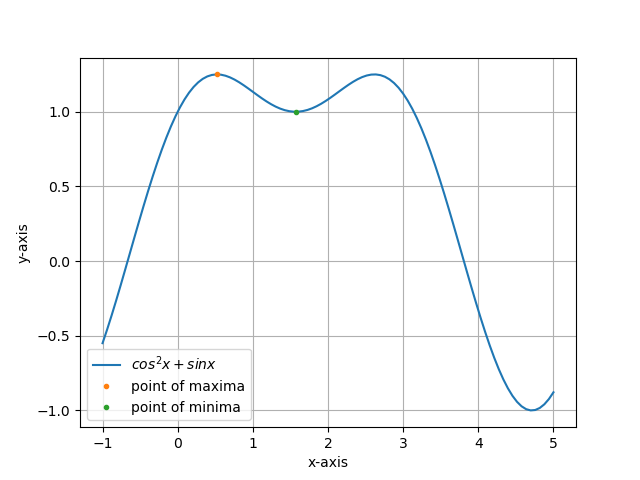
\includegraphics[width=\columnwidth]{12/6/6/14/figs/opt.png}
		\caption{}
		\label{fig:12/6/6/14}
  	\end{figure}
\iffalse

\section{Solution}
\begin{flushleft}
Given function is,\\
\end{flushleft}
\begin{equation}
    f(x)=\cos^2x + \sin x
\end{equation}
\subsection{Calculation using normal differentiation}
\begin{flushleft}
Differentiating (1) yields,
\end{flushleft}
\fi
The derivative of the given function is
\begin{align}
\nabla f(x) = \cos x-2\sin x \cos x 
\end{align}
\iffalse

\noindent Calculating the critical points:
$ \nabla f(x) = 0 $

\begin{equation}
\implies \cos{x} = 0 
\end{equation}
\begin{equation}
\implies -2\sin{x} + 1 = 0
\end{equation}
Therefore, the critical points are 

\begin{equation}
\frac{\pi}{6},\quad\frac{5\pi}{6},\quad\frac{\pi}{2}
\end{equation}

\textbf{1.1.1 Finding absolute maximum and minimum} 
Since given interval is $x \in [0,\pi]$ 

\begin{table}[h]
\centering
\large
\begin{tabular}{|l|l|}
\hline
\textbf{value of x} & \textbf{value of} \\ \hline
At x =0             & 1                 \\ \hline
At x =$ \frac{\pi}{6}$            & $\frac{5}{4}$            \\ \hline
At x =  $ \frac{\pi}{2}$            & 1                 \\ \hline
At x =  $ \frac{5\pi}{6}$            & $\frac{5}{4}$             \\ \hline
at x =       $\pi$       & 1                 \\ \hline
\end{tabular}
\end{table}

Hence, 
\begin{align}
\text{absolute maximum} & =  \frac{5}{4}\\
\text{absolute minimum} & = 1
\end{align}

\subsection{Calculation of Maxima using gradient ascent algorithm}
\fi
The 
maxima is calculated by
\begin{align}
x_{n+1} = x_n + \alpha \nabla f(x_n) 
\\
 &= x_n + \alpha \brak{cosx_n-2sinx_ncosx_n}
\end{align}
where 
\begin{enumerate}
	\item $x_0=0.5$ 
	\item $\alpha=0.001$ 
	\item precision $= 0.00000001$ 
\end{enumerate}
yielding
    \begin{align}
	    f_{max} = 1.25, 
 x_{max}        = 0.52.
    \end{align}
    \iffalse
    
\begin{figure}[h!]
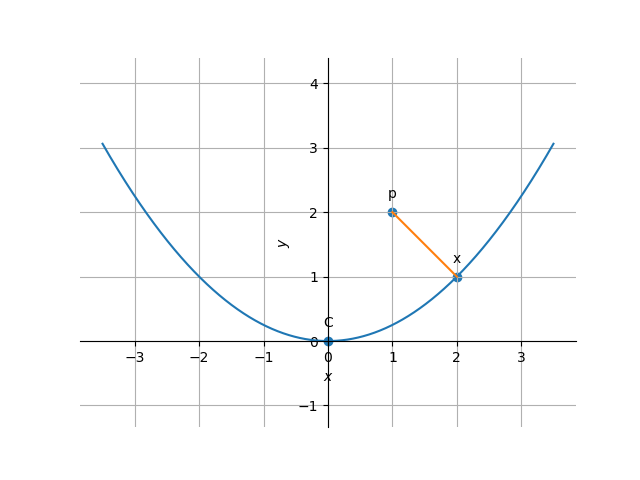
\includegraphics[scale=0.55]{opt.png}
\caption{The function f(x) with maxima and minima points}
\end{figure}        

\subsection{Calculation of Minima using gradient descent algorithm}
To find: 
\begin{align}
\min_{x} f(x)
\end{align}  
Given:
\begin{align}
f(x) = \cos^2x + \sin x,\quad x \in [0,\pi] 
\end{align}
\fi
The 
minima  is found by 
\begin{align}
	x_{n+1} &= x_n - \alpha \nabla f(x_n)
\\
 &= x_n - \alpha \brak{cosx_n-2sinx_ncosx_n}
\end{align}
\iffalse
where \\
1)$x_0=0.5$ \\
2)$\alpha=0.001$ \\
3)precision $= 0.00000001$ \\
values obtained using python are:
    \begin{align}
        \boxed{\text{Minima} = 1 }\\
        \boxed{\text{Minima Point} = 1.57}
    \end{align}

\end{document}
\fi


\end{enumerate}
